\chapter[Identificación de Métodos Generadores de Objetos]{Identificación de Métodos Generadores de Objetos}
\label{cap:builders}

\cacho{1 - Cambiar putos por observadores en todos lados}
\cacho{2 - terminar las citas}
\cacho{1 - }
\cacho{1 -}

% Primera etapa
\section{Ejemplo Motivador}

\begin{table}[]
\centering
{\scriptsize
\begin{tabular}{|l|l|l|}
\hline
No. & Nombre del Método & Puro? \\
\hline
0 & NCL() & no \\
1 & NCL(int) & no \\
2 & NCL(Collection) & no \\
3 & add(Object) & no \\
4 & add(int,Object) & no \\
5 & addAll(Collection) & no \\
6 & addAll(int,Collection) & no \\
7 & addFirst(Object) & no \\
8 & addLast(Object) & no \\
9 & clear() & no \\
10 & contains(Object) & sí \\
11 & containsAll(Collection) & sí \\
12 & equals(Object) & sí \\
13 & get(int) & sí \\
14 & getFirst() & sí \\
15 & getLast() & sí \\
16 & indexOf(Object) & sí \\
17 & isEmpty() & sí \\
18 & iterator() & no \\
19 & lastIndexOf(Object) & sí \\
20 & listIterator() & no \\
21 & listIterator(int) & no \\
22 & remove(int) & no \\
23 & remove(Object) & no \\
24 & removeAll(Collection) & no \\
25 & removeFirst() & no \\
26 & removeLast() & no \\
27 & retainAll(Collection) & no \\
28 & set(int,Object) & no \\
29 & size() & sí \\
30 & subList(int,int) & si \\
31 & toArray() & sí \\
32 & toArray(Object[]) & sí \\
33 & toString() & sí \\
\hline
\end{tabular}
}
\caption{API de NodeCachingLinkedList de Apache}
\label{tab:ncl-api}
\end{table}


Para comprender mejor la definición de métodos generadores de objetos, motivaremos la misma mediante un ejemplo de una API real. La estructura de datos NodeCachingLinkedList (NCL) de Apache \cite{apache} está diseñada como una lista principal, circular y doblemente enlazada, que almacena los elementos de la colección. Además, incluye una lista secundaria simplemente enlazada que actúa como caché para nodos eliminados de la lista principal. Esta caché permite reutilizar los nodos almacenados, mejorando el rendimiento en aplicaciones donde las operaciones de inserción y eliminación son frecuentes. Gracias a esta optimización, NCL reduce significativamente la sobrecarga asociada a la asignación de memoria y a la recolección de basura. 

La API de NodeCachingLinkedList incluye un conjunto de métodos (ver tabla \ref{tab:ncl-api}) que permiten construir, modificar y consultar la colección. Esta API combina funcionalidades típicas de listas enlazadas con optimizaciones adicionales relacionadas con el reuso de nodos en la caché. Los métodos pueden clasificarse en tres categorías principales según su función: 

\begin{itemize}
    \item \textbf{Métodos constructores:}
    Los métodos constructores (líneas 0-2 en la Tabla~\ref{tab:ncl-api}) permiten crear nuevos objetos del tipo. Estos son:
    \begin{itemize}
        \item \texttt{NCL()}: Crea una lista vacía.
        \item \texttt{NCL(int)}: \cacho{Define el tamaño máximo permitido para la lista caché}
        \item \texttt{NCL(Collection)}: Crea una lista nueva que contiene todos los elementos de una colección dada.
    \end{itemize}
    \item \textbf{Métodos modificadores:}
    Estos métodos permiten agregar, eliminar o modificar elementos de la lista. Algunos ejemplos son:
    \begin{itemize}
        \item \texttt{add(Object)}: Agrega un elemento al final de la lista principal \cacho{y no se modifica la lista cache }
        \item \texttt{addFirst(Object)} y \texttt{addLast(Object)}: Insertan elementos al principio o al final de la lista principal \cacho{y no se modifica la lista cache}
        \item \texttt{remove(int)} y \texttt{remove(Object)}: Eliminan elementos de la lista por índice o por valor. El nodo eliminado se inserta en la lista cache de la estructura.
        \item \texttt{clear()}: Vacía la lista principal y  \cacho{se insertan los nodos en la lista cache}
        \item \texttt{set(int, Object)}: Modifica el elemento en una posición específica de la lista.
    \end{itemize}
    \item \textbf{Métodos observadores:}  
    Estos métodos permiten inspeccionar el estado de la lista sin modificarla:
    \begin{itemize}
        \item \texttt{contains(Object)}: Verifica si un elemento está presente.
        \item \texttt{get(int)}, \texttt{getFirst()} y \texttt{getLast()}: Recuperan elementos según su posición.
        \item \texttt{size()}: Retorna el número de elementos en la lista.
        \item \texttt{toArray()}: Crea un nuevo arreglo con todos los elementos de la lista.
    \end{itemize}
\end{itemize}

\noindent
A partir de esta API, los objetos de \emph{NodeCachingLinkedList} pueden construirse utilizando secuencias de operaciones que combinan los métodos constructores y los modificadores. Por ejemplo, una lista inicializada con \texttt{NCL()} puede llenarse mediante llamados consecutivos a \texttt{add(Object)} o \texttt{addAll(Collection)}, mientras que los métodos \texttt{remove(Object)} y \texttt{clear()} permiten vaciar la lista principal y crear elementos en la lista cache, según sea necesario.

La Figura~\ref{fig:ncl-instances-intro} muestra tres posibles instancias de NodeCachingLinkedList que pueden construirse utilizando exactamente dos nodos. A continuación, se presentan las secuencias de métodos generadores que permiten construir cada una de las configuraciones:


\begin{figure}[H]
    \centering
    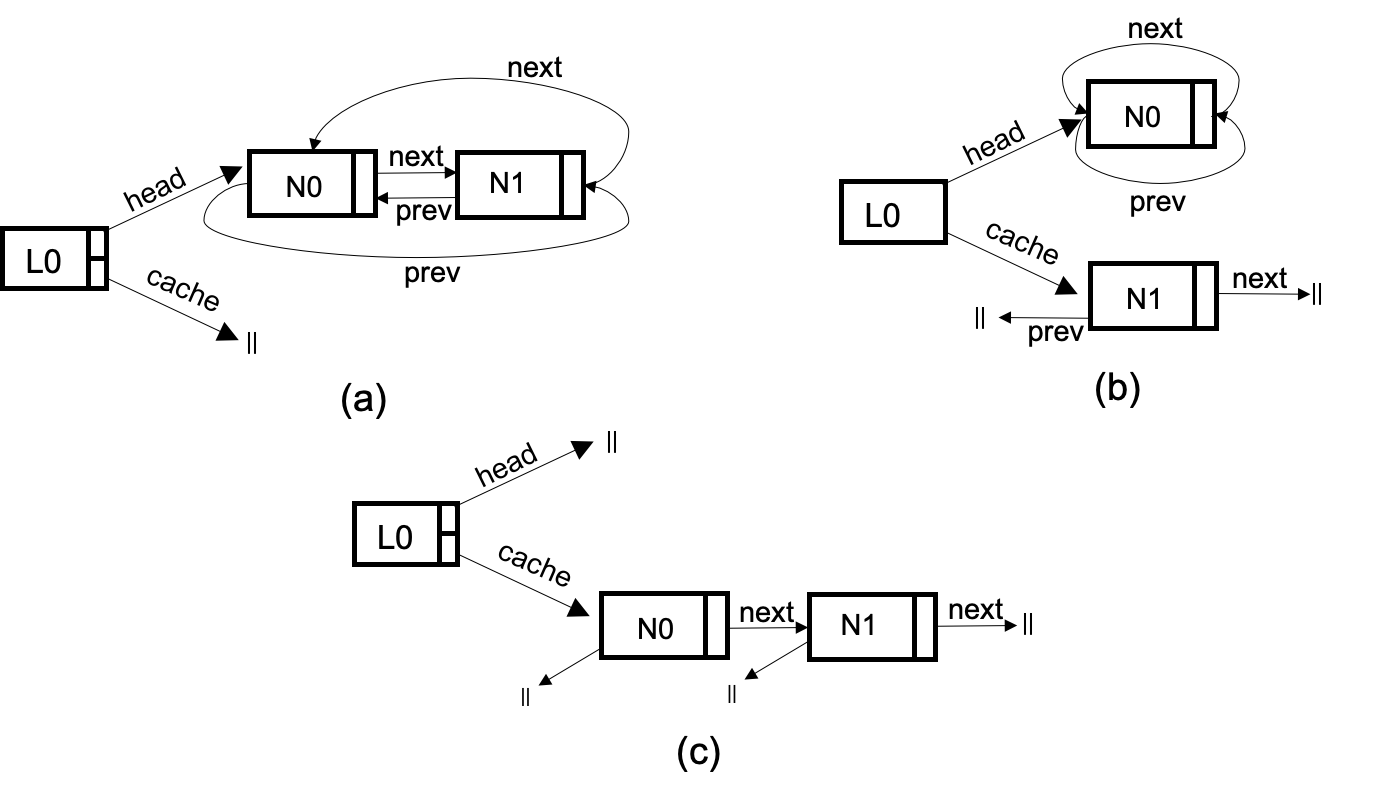
\includegraphics[width=0.85\textwidth]{images/NCL-instances.png}
    \caption{Tres instancias de NodeCachingLinkedList con exactamente dos nodos.}
    \label{fig:ncl-instances-intro}
\end{figure}

\begin{itemize}
    \item Figura (a):  
    Esta instancia se construye mediante la adición secuencial de dos nodos a la lista principal:
    \newline
    \begin{lstlisting}[numbers=none,label=fig:NCLbuilders_a,xleftmargin=0pt]
    (0)  NodeCachingLinkedList()
    (7)  addFirst(Object)
    (7)  addFirst(Object)
    \end{lstlisting}

    \item Figura (b):  
    Esta instancia se logra agregando un nodo a la lista principal y luego eliminarlo para que sea insertado en la cache:
    \newline

    \begin{lstlisting}[numbers=none,label=fig:NCLbuilders_b, xleftmargin=0pt]
    (0)  NodeCachingLinkedList()
    (7)  addFirst(Object)
    (25) removeFirst()
    \end{lstlisting}

    \item Figura (c): 
    Esta instancia se genera añadiendo dos nodos al inicio y luego eliminándolos secuencialmente para que se inserten en la lista cache:
    \newline

    \begin{lstlisting}[numbers=none,label=fig:NCLbuilders_c, xleftmargin=0pt]
    (0)  NodeCachingLinkedList()
    (7)  addFirst(Object)
    (7)  addFirst(Object)  
    (25) removeFirst()
    (25) removeFirst()
    \end{lstlisting}

\end{itemize}


\pp{Estaría bueno tener las secuencias de métodos que llevan de una lista a la otra en la figura. Y de paso esto da una idea intuitiva de qué serían los builders}

\section{Métodos Generadores de Objetos y sus Propiedades}

%\pp{Definición de generadores de objetos}
Notar que, a pesar de que la API de NCL es muy compleja, como se observa en la Tabla~\ref{tab:ncl-api}, no todos los métodos son necesarios para construir objetos. Por ejemplo, combinaciones de los métodos mostrados en la Figura~\ref{fig:NCLbuilders}, con los parámetros adecuados, son suficientes para generar cualquier instancia de NCL.
\newline
\begin{lstlisting}[numbers=none,label=fig:NCLbuilders, caption=Conjunto de métodos generadores de objetos para NCL]
  (0)  NodeCachingLinkedList()
  (7)  addFirst(Object)
  (25) removeFirst()
\end{lstlisting}

Una vez inicializada la instancia de NCL con el constructor, se pueden insertar elementos en la lista utilizando el método \texttt{addFirst}. Adicionalmente, el método \texttt{removeFirst} permite crear instancias que posean nodos en la lista caché. 

De esta manera, los métodos de la Figura~\ref{fig:NCLbuilders} conforman un conjunto \emph{suficiente de métodos generadores de objetos}, es decir, son conjuntos de métodos que permiten generar todos los objetos posibles de NCL. Por simplicidad, llamaremos \emph{generadores de objetos} a estos métodos.

Notar que pueden existir distintos subconjuntos suficientes de generadores de objetos, como por ejemplo los que se muestran en las Figuras~\ref{fig:NCLbuilders2} y~\ref{fig:NCLnoMin1}. 
\newline
\begin{lstlisting}[numbers=none,label=fig:NCLbuilders2, caption=Otros métodos generadores de objetos, frame=tb , basicstyle=\scriptsize, xleftmargin=0pt]
  (0)  NodeCachingLinkedList()
  (3)  add(Object)
  (25) removeFirst()
\end{lstlisting}


En particular, la Figura~\ref{fig:NCLnoMin1} contiene métodos \emph{superfluos}, es decir, métodos que pueden quitarse sin perder la propiedad de suficiencia del conjunto resultante. Por ejemplo, podemos eliminar \texttt{remove(Object)} y los métodos restantes siguen siendo generadores de objetos suficientes (similarmente, podríamos eliminar \texttt{removeFirst()}). 
\newline

\begin{lstlisting}[numbers=none,label=fig:NCLnoMin1, caption=Métodos generadores de objetos suficientes pero no minimales, captionpos=b, frame=tb , xleftmargin=0pt, basicstyle=\scriptsize]
  (0)  NodeCachingLinkedList()
  (7)  addFirst(Object)
  (3)  remove(Object)
  (25) removeFirst()
\end{lstlisting}

Estamos interesados en conjuntos de métodos generadores de objetos \emph{minimales}, es decir, en conjuntos generadores de objetos suficientes con la menor cantidad posible de métodos. En otras palabras, los generadores de objetos son minimales si la exclusión de cualquiera de los métodos hace imposible la creación de ciertas instancias del módulo.
Así, las Figuras~\ref{fig:NCLbuilders} y ~\ref{fig:NCLbuilders2} muestran ejemplos de generadores de objetos suficientes y minimales.

Notar que muchos métodos en la tabla \ref{tab:ncl-api} están marcados como observadores (columna Obs?), lo que significa que no modifican los objetos sobre los que operan, ni son útiles para crear nuevos objetos. Notar que debido a esto los métodos observadores siempre son superfluos y nunca deben incluirse en un conjunto de generadores de objetos minimal. Por esta razón, nuestros enfoques de identificación de métodos generadores intentan reconocerlos de antemano y descartarlos.

Por último, observamos que cuanto más fáciles de instanciar sean los parámetros de una rutina, usualmente la rutina será más eficiente de utilizar en el contexto de un análisis de programas (por ejemplo, para generar entradas para testing). Por ejemplo, entre las alternativas de rutinas para insertar datos en
la lista principal de NCL (ver Tabla~\ref{tab:ncl-api}), \texttt{add(int,Object)} recibe más parámetros que los otros tres métodos posibles. En cambio, \texttt{add(Object)}, \texttt{addFirst(Object)}, \texttt{addLast(Object)} toman un único parámetro. Si bien cualquiera de estas rutinas sirve para generar los mismos objetos de NCL, hay más formas de invocar a \texttt{add(int,Object)}. Esto usualmente redunda en una pérdida de eficiencia en la construcción de objetos por parte de un análisis automático de programas. Similarmente, elegiremos métodos con parámetros más simples (por ejemplo, parámetros de tipo primitivo), que otros con parámetros más complejos (por ejemplo, parámetros de tipo referencia) siempre y cuando los métodos permitan construir los mismos objetos.

De la discusión anterior se desprende que preferimos los métodos con menor número de parámetros, y con parámetros más fáciles de instanciar en los generadores de objetos (siempre que se mantengan las propiedades de suficiencia y minimalidad de los generadores). En nuestro ejemplo anterior, elegiremos \texttt{add(Object)} (o \texttt{addFirst(Object)} o \texttt{addLast(Object)}) en lugar de \texttt{add(int,Object)} como parte de un conjunto suficiente y minimal de generadores de objetos.

Para concluir esta sección, es importante destacar que identificar manualmente un conjunto suficiente y minimal de métodos generadores de objetos es una tarea difícil y trabajosa, que requiere inspeccionar minuciosamente el código fuente del módulo y las formas en las que los métodos interactúan entre sí para generar objetos. Esto se dificulta aún más cuando los módulos cuentan con APIs ricas, como en nuestro ejemplo motivador (ver Tabla~\ref{tab:ncl-api}). 
Para facilitar la tarea del desarrollador, en las secciones siguientes proponemos enfoques automáticos para identificar conjuntos de métodos generadores de objetos.

%\pp{Para que servirían los generadores de objetos}

%Los métodos generadores de objetos son aquellos métodos específicos diseñados para crear, modificar y retornar objetos de una clase en particular. Este conjunto de método es capaz de generar cualquier configuración posible de la API. La identificación manual de estos métodos requiere un análisis exhaustivo de la lógica y el código de la API. 
% 2- Por qué es importante

%En sistemas de software grandes y complejos, los objetos suelen tener múltiples atributos y configuraciones específicas que deben recrearse para realizar pruebas efectivas. Los métodos generadores son especialmente útiles en este contexto, ya que permiten crear objetos mediante una combinacion de métodos que simplifican la generación de configuraciones específicas de una API. Sin estos métodos generadores, el uso directo de todos los métodos de la API puede resultar en la creación de objetos redundantes o configuraciones innecesarias, complicando el análisis y aumentando el costo computacional. Herramientas como \emph{Randoop} o \emph{JPF} (\cacho{ver referencias}) pueden beneficiarse de estos métodos al generar secuencias más eficientes y relevantes.

%Por ejemplo, al recrear configuraciones de la API sin métodos generadores, se puede observar cómo se generan objetos redundantes y combinaciones innecesarias 



%Además, estos subconjuntos de métodos son clave en las pruebas unitarias, ya que permiten crear configuraciones específicas necesarias para probar diferentes escenarios y casos de uso. Dichas configuraciones solo pueden generarse a través de combinaciones específicas de llamadas a los métodos generadores de objetos.

%La priorización de métodos generadores tiene aplicaciones prácticas importantes:

%\begin{enumerate}
%    \item \textbf{Eliminación de redundancias en \emph{Randoop}:} Al priorizar subconjuntos específicos de métodos, se reducen las redundancias en las secuencias generadas, optimizando el proceso de pruebas y reduciendo el número de casos innecesarios sin comprometer la cobertura.

%    \item \textbf{Drivers para pruebas parametrizadas con \emph{Symbolic PathFinder} (SPF):} Los métodos generadores seleccionados pueden utilizarse para crear \emph{drivers} que exploren rutas en pruebas parametrizadas, proporcionando configuraciones iniciales relevantes y maximizando el análisis simbólico.
%\end{enumerate}

%En resumen, los métodos generadores no solo simplifican la creación de objetos y configuraciones específicas, sino que también permiten mejorar la eficiencia y efectividad de las pruebas automatizadas en herramientas avanzadas.



%Es importante destacar que estas configuraciones deben estar limitadas para poder crearlas de manera eficiente y efectiva. Para lograr esto, se introduce el concepto de "scope", que representa el límite en el número de objetos y rangos para los tipos de datos, como se describe en \cite{jackson2006, frias2005dynalloy}.
%\cacho{Chequear la cita, lo saque del paper de Efficient Bounded Model Checking of Heap-Manipulating Programs using Tight Field Bounds}. La justificación para utilizar conjuntos acotados de objetos es similar a la hipótesis de alcance de la cota pequeña \cite{Andoni:2003}. Si un conjunto de métodos no puede utilizarse para construir objetos pequeños que permitan diferenciarlo de otro conjunto de métodos, es poco probable que estos dos conjuntos puedan distinguirse con objetos más grandes.

% \pp{Características de generadores de objetos: suficientes y minimales}
% En el contexto de una API, el conjunto de métodos generadores de objetos debe tener las propiedades de ser suficiente y minimalista para garantizar un manejo eficiente y completo de las configuraciones de objetos posibles.

% La propiedad de ``suficiente'' implica que este conjunto de métodos debe ofrecer todas las opciones y parámetros necesarios para configurar completamente un objeto de la API. En otras palabras, con estos métodos, los usuarios deben poder generar cualquier configuración deseada de objetos dentro de la API. Esta característica es fundamental, ya que garantiza que el subconjunto de métodos generadores sea competente y abarque todas las posibilidades que la API puede ofrecer. La ausencia de cualquier método de este conjunto podría significar que exista al menos una configuración de la API que no se pueda recrear o generar.

% Por otro lado, la propiedad de ``minimal'' es igualmente importante que la propiedad de suficiencia. Al referirnos a que los métodos deben ser minimalistas, nos referimos a que deben ser los más simples \cacho{No se si es la palabra acorde} y el conjunto debe tener la menor cantidad posible de métodos. Esto quiere decir, que cada método debe cumplir una función específica y claramente definida, sin redundancia innecesaria. Especialmente en situaciones donde los objetos pueden tener múltiples atributos o propiedades, la falta de la propiedad de minimalismo del subconjunto de métodos puede generar una explosión de combinaciones de los mismos, dificultando el proceso de generación.



\pp{Dejarlo para cuando terminemos el resto de este capítulo.}
\cacho{Agregar un ejemplo visual, Arbolito y explicarlo} \pp{Quizás esto sirva para explicar la explosión de combinaciones de métodos en los análisis de programas? Hay que pensarlo..} 
\pp{Pablo: Builders usage in program analyses? Now or later? We'll see...}
% Manually selecting sufficient and minimal builders is not an easy task: it requires a thorough analysis of the available routines and a deep understanding of the program semantics. This is especially hard for programs with rich APIs, where there are many routines and a lot of redundancy in the API (see Section \ref{sec:motivating}). We propose an automated approach for identifying such a sufficient and minimal set of builders, based on an evolutionary algorithm that searches for a minimal set of routines that is capable of generating the maximum number of different (bounded) objects (i.e., $BE(M, k)$). Moreover, our evolutionary approach also takes into account other characteristics of the builders, such as the number and complexity of their parameters, so that ``simpler'' routines are favored in the search. 
%The goal is to choose builders that can be more easily and more efficiently used by the subsequent program analyses.


% Pablo: Scope?



\section{Definiciones preliminares}
\label{sec:preliminares}


% Intro
\cacho{Poner las citas}
En este capítulo, nos enfrentamos al desafío de identificar un conjunto suficiente y mínimo de generadores de objetos a partir de la API de un módulo. Nos enfrentamos a un problema de optimización, donde apuntamos a encontrar el mejor estado según una función objetivo. Esta definición es la de los algoritmos de búsqueda local \cite{Russell:2009}. Para abordar este problema desarrollamos dos algoritmos de búsqueda, cada uno con su enfoque único. Estos algoritmos nos permiten explorar el espacio de búsqueda de manera eficiente y efectiva.

El primer algoritmo que presentamos es un enfoque basado en algoritmos genéticos, que utiliza principios inspirados en la evolución biológica \cite{}
%, este algoritmo se enfoca en generar conjuntos de métodos generadores que puedan dar lugar a configuraciones más grandes y diversas de objetos. 
La naturaleza basada en la evolución de este enfoque permite encontrar soluciones prometedoras y adaptarse a diferentes situaciones.

El segundo algoritmo que proponemos es un enfoque \emph{greedy}, específicamente una variante de un algoritmo de ascenso de colinas \cite{}. Este enfoque se centra en mejorar iterativamente un conjunto inicial de métodos generadores mediante la adición de métodos.
%, buscando siempre mejorar la calidad del conjunto en términos de eficiencia en cuanto a los objectos generados y la cobertura que se logra utilizando estos objectos sobre la API bajo test.

%Por último, presentamos un algoritmo basado en la idea de particionar los subconjuntos de métodos de la API en "clases de equivalencias" según los objetos que construyen. Esta estrategia nos permite agrupar métodos con propiedades similares y seleccionar conjuntos de métodos más cohesivos y efectivos.

Cada uno de estos algoritmos ofrece ventajas y desventajas en términos de rendimiento y precisión. Nuestra investigación se centró en comparar y evaluar estos algoritmos en diferentes casos de estudio para determinar cuál de ellos se adapta mejor a la tarea de identificar conjuntos suficientes y mínimos de generadores de objetos.

% Para abordar estos desafíos planteados, a continuación se proponen dos enfoques para seleccionar automáticamente un conjunto suficiente y minimal de métodos generadores de objetos a partir de una API. El primero es un enfoque \emph{greedy}, basado en \emph{hill climbing}. El segundo enfoque utiliza algoritmos genéticos. En la próxima sección, explicaremos en detalle cada uno de estos enfoques y su implementación.

Por simplicidad, a partir de esta sección llamaremos generadores de objetos a aquellos que cumplan con las propiedades de suficiencia y minimalidad, ya que estamos interesados en identificar generadores de objetos con estas características.

% Observadores que es compartido por todos los algoritmos

\subsection{Identificación de métodos observadores}

 Los métodos observadores cumplen un papel fundamental en la API, ya que permiten inspeccionar el estado de un objeto. Estos métodos se caracterizan por no modificar el estado interno del objeto en cuestión. En otras palabras, su ejecución no altera ninguno de los atributos del objeto.
  También pueden usarse para verificar el estado de un objeto antes de realizar una operación que podría modificarlo.
 Por ejemplo, antes de eliminar un elemento de una lista, el método \texttt{isEmpty} de la lista puede ser utilizado para verificar si la lista contiene elementos. Si está vacía, se evita intentar una operación inválida.

Se puede observar en el código de la Figura \ref{fig:emptyObs} que las funciones \emph{isEmpty} y \emph{size} de la clase NodeCachingLinkedList (NCL) son métodos observadores.  Estos métodos no modifican ningún atributo de la clase NCL.
 
\begin{lstlisting}[language=Java, label=fig:emptyObs, caption=Algunos métodos observadores de la clase NCL. Se observa que no modifican el estado de NCL., captionpos=b, frame=tb, float=t]
public class NodeCachingLinkedList {
    Node head;
    int size;
    /**
      Devuelve verdadero si la lista esta vacia. 
    */ 
    public boolean isEmpty() { 
        return head == null; 
    }
    
    /**
      Devuelve el tamano de la lista. 
    */ 
    public int size() { 
        return size; 
    }
    
    // ... código omitido ...
}
\end{lstlisting}


 En el ejemplo motivador presentado en la sección anterior y en la Tabla \ref{tab:ncl-api} se puede ver que existen muchos métodos clasificados como observadores. 
Antes de ejecutar cualquiera de nuestros algoritmos, resulta fundamental identificar los métodos observadores. La razón principal es que estos métodos no contribuyen en la creación de nuevos objetos, ya que no sirven para construir objetos ni para modificar el estado de los objetos existentes. Por ende, no tienen ninguna utilidad en el contexto de los algoritmos de búsqueda de generadores de objetos.

Para automatizar la identificación de métodos observadores, hemos utilizado una herramienta de análisis estático, \emph{Infer} \footnote{https://fbinfer.com/}, desarrollada por Facebook. \emph{Infer} ofrece funcionalidades avanzadas que permiten analizar código fuente y clasificar métodos como observadores \cite{Huang:2012} (también denominados métodos puros en la bibliografía \cite{Huang:2012}). \emph{Infer} implementa la identificación de observadores mediante un análisis estático del código de los métodos \cite{}. Si bien el análisis de \emph{Infer} puede ser impreciso en algunos casos y generar falsos negativos (clasificar métodos como no observadores cuando si lo son), en nuestros experimentos \emph{Infer}  identifica una buena proporción de los observadores de las APIs, lo que reduce significativamente el espacio de búsqueda de nuestros algoritmos.


% Entre las ventajas de utilizar \emph{Infer} se incluyen:

% \begin{itemize}
% \item \textbf{Eficiencia:} Automatiza el proceso de clasificación, ahorrando tiempo y esfuerzo manual.
% \item \textbf{Precisión:} Reduce el riesgo de errores humanos al identificar métodos irrelevantes para ciertos análisis.
% \item \textbf{Compatibilidad:} Es compatible con varios lenguajes de programación y puede integrarse en flujos de desarrollo modernos.
% \end{itemize}


\cacho{Por ejemplo, al analizar la API de NCL con \emph{Infer}, el resultado que obtenemos es el que se encuentra en la columna "Puro?" de la tabla \ref{tab:ncl-api}}

De esta manera, \emph{Infer} es utilizado como paso previo a la ejecución de nuestros algoritmos. Los métodos reportados como observadores por \emph{Infer} se descartan antes de comenzar la búsqueda de métodos generadores de objetos.


% 1- estados o configuraciones del problema
\subsection{Estados}
\label{sec:estados}
En el contexto de los algoritmos de búsqueda local, los estados representan las diferentes configuraciones o situaciones posibles dentro del problema que se está resolviendo. Cada estado corresponde a un elemento en el espacio de búsqueda, definido como el conjunto de todas las posibles combinaciones o configuraciones que el algoritmo puede explorar para encontrar una solución.

La representación de los estados es un elemento clave para el éxito de los algoritmos de búsqueda, ya que determina el tamaño del espacio de búsqueda. 
% Una representación adecuada debe cumplir con los siguientes criterios:
% \begin{itemize}
%     \item \textbf{Relevancia:} Capturar todas las características esenciales del problema sin incluir información redundante o innecesaria.
%     \item \textbf{Eficiencia:} Permitir operaciones rápidas de expansión, evaluación y manipulación durante la búsqueda.
%     \item \textbf{Escalabilidad:} Adaptarse a problemas de mayor complejidad sin introducir un sobrecosto computacional significativo.
% \end{itemize}
Una representación demasiado compleja puede hacer que el algoritmo sea computacionalmente costoso y lento, mientras que una representación demasiado simplificada puede llevar a la pérdida de información importante, reduciendo la capacidad del algoritmo para encontrar soluciones óptimas.

%La codificación del espacio de búsqueda implica definir cómo se representan los estados y cómo se generan nuevos estados durante la exploración. 
En nuestros algoritmos de búsqueda, los estados están compuestos por subconjuntos de métodos de una API. Para representar estos subconjuntos, utilizamos vectores booleanos, donde cada posición en el vector indica si un método específico está incluido o no en el conjunto.

Como vimos en la tabla \ref{tab:ncl-api}, \texttt{NCL}, tiene un total de 34 métodos. Sin embargo, no todos estos métodos son relevantes para nuestros algoritmos. Por ejemplo, los métodos observadores deben excluirse del análisis ya que no contribuyen a la construcción de objetos. Esto reduce el número total de métodos considerados, lo que a su vez reduce significativamente el espacio de búsqueda.

Después de excluir los métodos puros, quedan 20 métodos relevantes en NCL. Estos métodos se enumeran desde 0 hasta 19 como se puede observar en la tabla \ref{tab:ncl-api-infer}. 
\begin{table}[h!]
\centering
{\scriptsize
\begin{tabular}{|l|l|}
\hline
No. & Nombre del Método \\
\hline
0 & NCL() \\
1 & NCL(int) \\
2 & NCL(Collection) \\
3 & add(Object) \\
4 & add(int,Object) \\
5 & addAll(Collection) \\
6 & addAll(int,Collection) \\
7 & addFirst(Object) \\
8 & addLast(Object) \\
9 & clear() \\
10 & iterator() \\
11 & listIterator() \\
12 & listIterator(int) \\
13 & remove(int) \\
14 & remove(Object) \\
15 & removeAll(Collection) \\
16 & removeFirst() \\
17 & removeLast() \\
18 & retainAll(Collection) \\
19 & set(int,Object) \\
\hline
\end{tabular}
}
\caption{API de NodeCachingLinkedList de Apache}
\label{tab:ncl-api-infer}
\end{table}

\pp{Acá hay que listar de nuevo los métodos de NCL en una tabla y enumerarlos. Así después se puede entender el vector. Sino no se sabe a qué posición corresponde cada cosa.}

La representación de los estados en nuestros algoritmos se realiza mediante vectores booleanos. Cada posición $i$ en el vector representa el $i$-ésimo método de la API:

\[
c = [g_1, g_2, \ldots, g_n]
\]

donde:
\begin{itemize}
    \item $g_i = 1$ si el $i$-ésimo método está incluido en el subconjunto representado por el estado.
    \item $g_i = 0$ si el método no está incluido.
\end{itemize}

Por ejemplo, un estado posible puede representarse como un vector de la siguiente forma:


\begin{figure}[H]
  \centering
  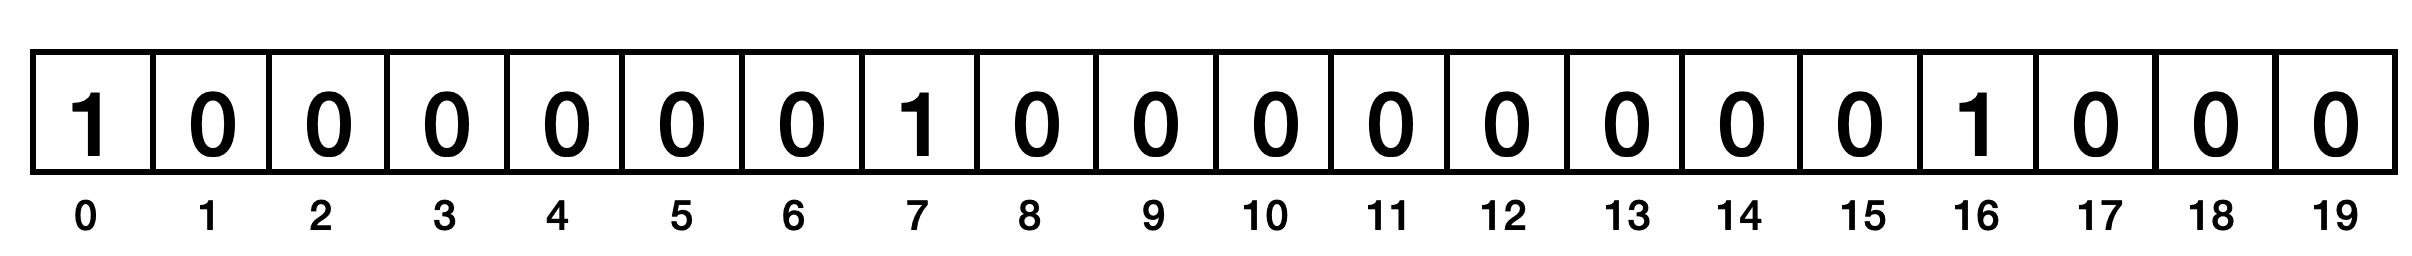
\includegraphics[width=1.0\textwidth]{images/cromosoma.png}
  \caption{Ejemplo de representacion de estado con un vector booleano}
  \label{fig:crossover}
\end{figure}

En este caso, las posiciones 0, 6 y 16 del vector están establecidas como verdaderas (según el orden asignado a los métodos de la API), mientras que las demás posiciones están establecidas como falsas. Esta configuración representa el subconjuto de métodos:
\newline

\begin{lstlisting}[numbers=none,label=fig:NCLnoMin1, caption=Métodos generadores de objetos que representa el cromosoma de la Figura 2, captionpos=b, frame=tb , xleftmargin=0pt, basicstyle=\scriptsize]
  (0)  NodeCachingLinkedList()
  (7)  addFirst(Object)
  (16) removeFirst()
\end{lstlisting}

\subsection{Funciones objetivo}
\label{sec:fitness}
% 2- función de valoración
% también denominada función de aptitud en algoritmos genéticos

Una función objetivo, también conocida como función de costo o función de valuación, es una función matemática que mide la calidad de una solución candidata dentro del espacio de búsqueda \cite{}. Esta función asigna un valor numérico a cada estado, indicando qué tan buena o deseable es el candidato con respecto al objetivo del problema.

El propósito de la función objetivo es guiar el proceso de búsqueda hacia la mejor solución posible. Dependiendo del problema, se busca maximizar o minimizar el valor de la función. En problemas de maximización, se priorizan los estados con valores más altos, mientras que en problemas de minimización, se favorecen aquellos con valores más bajos.

La función objetivo es una parte fundamental de los algoritmos de búsqueda local. Estos algoritmos utilizan la función objetivo para evaluar y comparar diferentes estados candidatos a medida que exploran el espacio de búsqueda en busca de la mejor solución posible.

En nuestros algoritmos, hemos desarrollado dos funciones objetivo distintas para guiar el proceso de búsqueda. Cada una de ellas tiene su enfoque único para evaluar y comparar diferentes configuraciones de métodos generadores de objetos.

Como el conjunto de objetos que se pueden construir con la API de un módulo es potencialmente infinito, las funciones objetivo definidas a continuación usan diferentes mecanismos para acotar el espacio de búsqueda.


\subsubsection{Generación Exhaustiva Acotada}
\label{sec:fitnessGE}

Dado un candidato $c$ que representa un subconjunto de métodos $M$ de la API, nuestra función de valuación intenta calcular una aproximación del número de objetos que se pueden construir utilizando combinaciones de métodos en $M$. Los candidatos con valores de aptitud más altos se estima que construyen más objetos que aquellos que tienen valores de aptitud más pequeños.

Así, la primera función objetivo propuesta evalúa la capacidad de generación de objetos de un candidato $c$ realizando una generación exhaustiva acotada \cite{Politano20} usando los métodos en $M$. La función objetivo asigna un puntaje a $c$ basándose en la cantidad de objetos únicos producidos durante la generación exhaustiva acotada. Esto refleja la diversidad de objetos que se pueden generar utilizando los métodos dados. Los subconjuntos de métodos que generan más objetos serán los candidatos preferidos para ser elegidos por nuestro algoritmo como generadores de objetos. Más adelante, analizaremos el caso en el que existe más de un subconjunto de generadores de objetos (como se discutió en la Sección \ref{}).
\cacho{referncia del capitlo}

Nuestro enfoque utiliza un generador exhaustivo acotado eficiente basado en métodos de la API \cite{Politano20}. Este generador se denomina BEAPI y es una de las contribuciones principales de este trabajo (ver Capítulo \ref{cap:beapi}).
Dado un conjunto de métodos $M$ en un candidato $c$, BEAPI explora todas las secuencias de métodos acotadas que se pueden construir usando métodos de $M$. La cota consiste de un número máximo $m$ de métodos dado por el usuario, y de un conjunto de valores primitivos empleados para instanciar los parámetros de tipo primitivo en los métodos en $M$ (e.g., enteros de \( 0 \) a \( k-1 \)). BEAPI utiliza cada uno de estos valores para instanciar cada parámetro de tipo primitivo (del tipo correspondiente). BEAPI cuenta la cantidad de objetos distintos creados por la ejecución de cada una de las secuencias exploradas. Así, para $M$ (y cotas $m$ y $k$) la función de valuación retorna el número de objetos generados por BEAPI usando $M$.

Como la cantidad de secuencias a explorar crece exponencialmente respecto de las cotas, BEAPI implementa distintas técnicas que le permiten podar significativamente el espacio de búsqueda y mejorar la eficiencia de la generación (usar el feedback de la ejecución para descartar secuencias inválidas, coincidencia de estado para evitar volver a generar repetidamente los mismos objetos, descartar secuencias que generen objetos de tamaño mayor al permitido por las cotas). Para obtener más información sobre las mismas y sobre BEAPI invitamos al lector a consultar el Capítulo \ref{cap:beapi}.

Notar que nuestra técnica se basa en una variante de la \emph{hipótesis de la cota pequeña}, ampliamente reconocida en el testing de software \cite{Andoni:2003,jackson2006, Abad13}. La hipótesis de la cota pequeña indica que la mayoría de las fallas pueden revelarse ejercitando el software bajo test con entradas de tamaño relativamente pequeño. Nuestra hipótesis es que si dos conjuntos de métodos $M_1$ y $M_2$ generan los mismos objetos acotados (para una cota relativamente pequeña), entonces es altamente probable $M_1$ y $M_2$ sirvan para generar los mismos objetos en un contexto no acotado. Esto fue validado empíricamente en todos nuestros casos de estudio.

\cacho{Pablo ver luego. Pensar en ejecucion simbolica que string es mas dificil que generar un int}

\begin{lstlisting}[label=fig:rankParameters,caption=Ranking con los tipos de parametros, captionpos=b,frame=tb, float=t]
Boolean=1
Integer,Char,Float,Double,String=2
Object=4
\end{lstlisting}

Como ya se discutió en esta Sección, buscamos un conjunto minimal de generadores de objetos, donde los métodos tengan parámetros tan simples como sea posible. Por lo tanto, la cantidad de objetos generados usando BEAPI es sólo un componente de la función objetivo. Dado un conjunto de métodos $M$, representado por un candidato $c$, la función objetivo $f$ devuelve un valor real conformado por tres componentes:

\[
f(M) = \langle O(M), R(M), C(M) \rangle
\]
Donde:

\begin{itemize}
    \item $O(M)$ (Objetos): Es el número de objetos generados por el conjunto de métodos $M$ usando generación exhaustiva acotada, para un scope fijo. Este componente es el más importante, ya que los siguientes componentes sólo se usan para decidir en caso de empate respecto de $O(M)$. Recordemos que los generadores de objetos a identificar deben ser siempre suficientes, por lo que la función objetivo siempre prioriza los métodos que generen un mayor número de objetos.
    \item $R(M)$ (Redundancia): Representa la diferencia entre el número total de métodos de la API ($M_t$) y la cantidad de métodos en $M$. Esto se utiliza para desempatar entre conjuntos de métodos que generan la misma cantidad de objetos, dando preferencia a aquellos conjuntos que contengan menos métodos. En otras palabras, este componente de la función busca identificar generadores de objetos minimales.
    \item $P(M)$ (Parámetros): 
    \cacho{Es una medida ponderada de la simplicidad de los parámetros de los métodos en $M$, definida como $w_1 \cdot PP(M)$, donde $w_1$ es un peso configurable. Este peso se puede observar en la tabla \ref{fig:rankParameters}. La funcion PP(M), devuelve los tipos de parametros que contiene el metodo M y de acuerdo al tipo se lo multiplica por el peso determinado. Este componente de $f$ se usa para desempatar entre conjuntos de métodos que generen la misma cantidad de objetos y tengan la misma cantidad de métodos.
    }
    \cacho{TENGO QUE DEFINIR MEJOR ESTO. ACA ES COMO EL MENOR Y EN CANTIDAD DE METODOS ES EL MAYOR. HAY QUE DEFINIR MEJOR ESTO }
\end{itemize}


A partir de esto, podemos definir un orden sobre esta función: 

\( f(M_1) = \langle O(M_1), R(M_1), P(M_1) \rangle \) 
\\
y 
\\
\( f(M_2) = \langle O(M_2), R(M_2), P(M_2) \rangle \) 
\newline

de la siguiente forma:

\[
f(M_1) > f(M_2) \quad \text{si y solo si:}
\]

\begin{enumerate}
    \item \( O(M_1) > O(M_2) \), o
    \item \( O(M_1) = O(M_2) \) y \( R(M_1) > R(M_2) \), o
    \item \( O(M_1) = O(M_2) \), \( R(M_1) = R(M_2) \), y \( P(M_1) > P(M_2) \).
\end{enumerate}

En otras palabras, se compara primero el número de objetos \( O(M_1) \) con \( O(M_2) \). Si son iguales, se compara la redundancia \( R(M_1) \) con \( R(M_2) \), y si ambos son iguales, se compara la complejidad de los parámetros \( P(M_1) \) con \( P(M_2) \).

Para ilustrar este concepto, consideremos los siguientes ejemplos.

En el primer caso, tenemos dos conjuntos de métodos:\\

\begin{lstlisting}[numbers=none,label=fig:NCLbuilders1, caption=Conjunto de métodos \( M_1 \)]
  NodeCachingLinkedList()
  addFirst(Object)
  removeFirst()
\end{lstlisting} 

\begin{lstlisting}[numbers=none,label=fig:NCLbuilders2, caption=Conjunto de métodos \( M_2 \)]
  NodeCachingLinkedList()
  addFirst(Object)
\end{lstlisting}

Obtenemos las siguientes triplas:

\[
f(M_1) = \langle 15, 17, 4 \rangle \quad \text{y} \quad f(M_2) = \langle 12, 18, 4 \rangle
\]

\cacho{Poner valores de objectos creados sacados de la parte experimental }

Dado que el conjunto \( M_1 \) genera más objetos (15 frente a 12), \( f(M_1) > f(M_2) \). Esto implica que \( M_1 \) es capaz de generar más instancias, mientras que \( M_2 \) no puede generar algunas que requieren métodos para agregar nodos a la lista cache.

En el segundo caso, ambos conjuntos generan la misma cantidad de objetos (15), pero \( M_4 \) tiene un método adicional:\\

\begin{lstlisting}[numbers=none,label=fig:NCLbuilders3, caption=Conjunto de métodos \( M_3 \)]
  NodeCachingLinkedList()
  addFirst(Object)
  removeFirst()
\end{lstlisting}

\begin{lstlisting}[numbers=none,label=fig:NCLbuilders4, caption=Conjunto de métodos \( M_4 \)]
  NodeCachingLinkedList()
  addFirst(Object)
  add(Object)
  removeFirst()
\end{lstlisting}

Las triplas resultantes son:

\[
f(M_3) = \langle 15, 17, 4 \rangle \quad \text{y} \quad f(M_4) = \langle 15, 16, 4 \rangle
\]

Aunque ambos conjuntos generan la misma cantidad de objetos, \( M_3 \) tiene una redundancia menor (16 frente a 17). Esto significa que \( f(M_3) > f(M_4) \), ya que \( M_3 \) contiene menos métodos redundantes.

En el tercer caso, los conjuntos tienen la misma cantidad de objetos y métodos, pero \( M_6 \) tiene más parámetros en el método \( add(int, Object) \):\\

\begin{lstlisting}[numbers=none,label=fig:NCLbuilders5, caption=Conjunto de métodos \( M_5 \)]
  NodeCachingLinkedList()
  addFirst(Object)
  removeFirst()
\end{lstlisting}

\begin{lstlisting}[numbers=none,label=fig:NCLbuilders6, caption=Conjunto de métodos \( M_6 \)]
  NodeCachingLinkedList()
  add(int, Object)
  removeFirst()
\end{lstlisting}

Obtenemos las siguientes triplas:

\[
f(M_5) = \langle 15, 17, 4 \rangle \quad \text{y} \quad f(M_6) = \langle 15, 17, 6 \rangle
\]

Ambos conjuntos generan la misma cantidad de objetos y tienen la misma redundancia, pero \( M_6 \) tiene parámetros más complejos (el método \( add(int, Object) \) tiene un parámetro adicional). Como resultado, \( f(M_6) > f(M_5) \), debido a que preferimos una menor complejidad en los parámetros.

\cacho{Deberia ser el Pesos total de parametros - el peso, pero es complicarla la explicacion. PENSAR COMO HACERLO}

\pp{Definir la función P teniendo en cuenta lo siguiente:
\texttt{o.M(p1: T1, p2: T2, ..., pm: Tm) -> P(M) = w(T1) + w(T2) + ... + w(Tm) = sum i=1..m w(Ti)}?
}



%Para este propósito, desarrollamos la herramienta BEAPI, que se discute con más detalle en el Capítulo \ref{cap:beapi}. En resumen, primero exploramos exhaustivamente todas las posibles combinaciones de secuencias de los métodos de $M$. Luego, utilizamos un conjunto fijo de valores primitivos (enteros del 0 a $k-1$) con los cuales probar nuestros métodos cuando requieren valores primitivos.

%En segundo lugar, descartamos las secuencias de métodos que crean objetos con más de $k$ objetos (de cualquier tipo) para evitar construir objetos más grandes de lo necesario. Para lograr esto, canonizamos los objetos generados por la ejecución de cada secuencia y descartamos la secuencia si algún objeto tiene un índice igual o mayor que $k$.

%En tercer lugar, ampliamos esta generación con coincidencia de estado. Esto se debe a que, en la generación de pruebas, a menudo hay muchas secuencias de pruebas que producen el mismo objeto. Por ejemplo, insertar en una colección y luego eliminar el mismo elemento resulta en muchos casos en exactamente la misma estructura antes de la inserción. Nuestro enfoque asume que las ejecuciones de rutinas son deterministas con respecto a sus entradas. Bajo esta suposición, se deduce que, para generar un conjunto exhaustivo acotado de estructuras, solo necesitamos guardar una secuencia de prueba para crear cada estructura diferente en el conjunto, y que todas las siguientes secuencias de prueba que generen la misma estructura se pueden descartar.


\subsubsection{Cobertura de código}
\label{sec:fitnessRandoop}

\cacho{secuencias con: builders* + no builders. Explicar esto}

\pp{No me acuerdo como funciona esta fitness. Para mi era correr randoop en 2 etapas, una con los métodos candidatos y después otra con toda la API. Tenemos que charlarlo. Otra cosa que no me cierra es qué devuelve la función. Para mi en teoría debería ser instrucciones cubiertas + ramas cubiertas. Aunque no esté implementado así no importa. Tampoco sé cuánto tiempo se corre Randoop para generar tests razonables.}

% Mergear con lo de abajo
La segunda función objetivo se enfoca en crear conjuntos de pruebas (test suites) utilizando los métodos de estado bajo evaluación y medir la cobertura que alcanzan estas test suites. La cobertura se refiere a cuántas líneas de código y cuántas ramas del programa son ejecutadas durante la ejecución de las pruebas. Esta métrica nos da una idea de qué tan bien cubren los conjuntos de pruebas las diferentes partes del programa, lo que nos permite evaluar la calidad y eficacia de los métodos generadores en términos de la cobertura lograda.

Los criterios de evaluación incluyen:
\begin{itemize}
    \item \textbf{Cobertura de líneas de código:} Porcentaje de líneas de código ejecutadas al correr los test suites.
    \item \textbf{Cobertura de ramas:} Porcentaje de decisiones (\textit{branches}) exploradas en el flujo de ejecución del programa.
\end{itemize}

Por ejemplo, si el conjunto de métodos seleccionados $M$ genera un test suite que cubre el 100 de las líneas de código y el 20 ramas de la API, la función objetivo podría combinar estas métricas en un puntaje compuesto que evalúe la calidad general del conjunto.

Este enfoque es especialmente útil en casos donde el objetivo es garantizar que los métodos seleccionados ejerzan la mayor cantidad posible de rutas de ejecución en la API.

Ambas funciones objetivo son utilizadas como criterios de evaluación en los algoritmos de búsqueda implementados. En algoritmos genéticos, la función objetivo actúa como la métrica de aptitud (\textit{fitness}), guiando la selección de los cromosomas más prometedores. En otros algoritmos de búsqueda, como los basados en escalada de colinas o recocido simulado (\textit{simulated annealing}), la función objetivo orienta el proceso de exploración del espacio de búsqueda.

En las siguientes subsecciones, detallaremos la implementación y funcionamiento de estas funciones objetivo, explicando cómo son utilizadas en nuestros algoritmos para guiar el proceso de búsqueda y seleccionar conjuntos de métodos generadores óptimos.

% END: Mergear con lo de abajo

En el contexto de nuestra tesis, hemos realizado modificaciones en la herramienta \emph{Randoop} descrita en la sección \ref{sec:feedback-directed-test-gen}.

Nuestras modificaciones se centran en dar prioridad a un subconjunto específico de métodos, representado en la sección anterior por el conjunto $M$. El objetivo de esta modificación es generar secuencias de pruebas que se enfoquen principalmente en la ejecución de estos métodos seleccionados. Sin embargo, es importante destacar que esto no implica excluir por completo otros métodos, ya que aún buscamos ejercitar la API en su totalidad para obtener una buena cobertura de todos los métodos.  \cacho{Solo le damos prioridad}

La motivación detrás de esta modificación radica en que los subconjuntos de métodos que obtienen una mayor cobertura de la API nos proporcionarán indicios valiosos sobre la calidad de dicho subconjunto. Por lo tanto, nuestra función de valoración tiene como objetivo maximizar la cobertura de ramas de la API bajo prueba, tal como se describe en la sección de preliminares \ref{sec:coverage}.

La función de valoración que utilizamos para evaluar la calidad de un candidato, que representa un conjunto de métodos $M$, se define como una tríupla al igual que la función de la sección anterior:

\[
f(M) = \langle Cob(M), R(M), C(M) \rangle
\]

Donde:

\begin{itemize}
    \item $Cob(M)$ (Cobertura de Ramas): Es el número de ramas cubiertas por las suites de prueba generadas por \emph{Randoop} utilizando el subconjunto de métodos $M$. Este componente tiene la mayor prioridad, ya que refleja directamente la efectividad de las pruebas al cubrir ramas específicas de la API.
    \cacho{Esta repetido, cambiar}
    \item $R(M)$ (Redundancia): Igual a la funcion de valoracion de la seccion de generador exhaustivo
    \item $C(M)$ (Complejidad): Tambien mantuvimos el mismo calculo que la funcion de valoracion del generador exhaustivo
\end{itemize}

En resumen, nuestras modificaciones en Randoop nos permiten priorizar un subconjunto de métodos durante la generación de secuencias de pruebas, y nuestra función de valoración se encarga de maximizar la cobertura de ramas de la API. Estas adaptaciones nos proporcionan una mejor comprensión de la calidad y efectividad de los subconjuntos de métodos generados.

\pp{Estaría bueno armar un ejemplo de la cobertura que da para dos conjuntos de builders diferentes.} 
\cacho{TODO: Ver los experimentos y poner algo aca}

\section{Algoritmos para la Identificación de Métodos Generadores de Objetos}
\label{sec:algorithms}

\pp{En algún lugar habría que meter un gráfico de cómo funciona la técnica a alto nivel. Creo que en alguna de las slides teníamos algo así.} 
\cacho{Poner algo de dibujitos algo sobre el flujo de la tecnicas}

\subsection{Algoritmo Genético}
\label{alg:approachGA}

En esta sección presentamos los detalles para la detección de los subconjuntos de métodos generadores de objetos utilizando un algoritmo genético. Cabe destacar que el algoritmo genético busca generadores de objetos suficientes y minimales.

\subsubsection{Población}

En el contexto de un algoritmo genético, la población se refiere a un conjunto de individuos o soluciones candidatas \cite{}. Cada individuo de la población representa una posible solución al problema que se está tratando de resolver. Para nuestro algoritmo representaremos los individuos como vectores de bits, como se describió en la Sección \ref{}. La población inicial se crea mediante  la generación aleatoria de $p$ individuos (vectores de bits), donde $p$ es un hiperparámetro del algoritmo genético.

En un algoritmo genético, la población evoluciona a lo largo de las generaciones a través de operaciones de selección, cruzamiento (\emph{cross-over}) y mutación \cite{}. En cada iteración del algoritmo, los individuos más aptos tienen más probabilidad de ser seleccionados para cruzarse y/o mutarse, y así crear nuevos individuos que a su vez formarán parte de la población de la siguiente generación. Con el tiempo, se espera que la población evolucione y mejore su aptitud en función del criterio de optimización establecido por la función objetivo.

En nuestro algoritmo, tenemos una población inicial de 100 individuos. Durante todo el proceso evolutivo, la población está limitada a un tamaño de 100 individuos. Cómo es típico para los hiperparámetros de los algoritmos genéticos determinamos el tamaño de la población empíricamente, probando distintos valores y utilizando el que mejor funcionaba en nuestros experimentos. 
%El método de prueba y error es comúnmente utilizado en computación evolutiva para definir los parámetros de búsqueda de manera adecuada. Es importante mencionar que si bien elegimos estos valores basándonos en los resultados de experimentos en un solo caso de estudio, luego utilizamos los mismos valores para el resto de los casos de estudio.

A medida que el algoritmo avanza, se aplican operadores genéticos como el cruzamiento y la mutación para crear nuevos individuos a partir de la población actual.

\subsubsection{Selección}

\cacho{Ver la palabra objetivo}

La selección en los algoritmos genéticos es el proceso de elegir qué individuos de la población actual participarán en la reproducción y darán lugar a la siguiente generación \cite{Goldberg:1989}. En este proceso, se otorgan mayores probabilidades de selección a los individuos más aptos, es decir, aquellos que tienen un mejor valor de la función objetivo \cite{Goldberg:1989} \pp{No sé si función objetivo es un buen nombre, en este contexto se usa fitness. Hay que ver cuál es la diferencia entre fitness y objetivo en el libro de AI}. \cacho{Llamar funcion objetivo pero aclarar en la seccion de genetico, que se suele llamarse fitness pero que usaremos funcion objetivo para simplificar los conceptos } La idea detrás de la selección es favorecer la transmisión de características deseables de los individuos más aptos a las generaciones futuras, para así mejorar gradualmente la calidad de las soluciones.

En nuestro enfoque, hemos utilizado un operador de selección tipo torneo (\emph{tournament}) \cite{Goldberg:1989}. Este enfoque funciona de la siguiente manera: se selecciona aleatoriamente un grupo de $t$ individuos de la población y se los pone a ``competir'' entre sí. El individuo más apto (con valor de la función objetivo) dentro de este grupo es seleccionado para participar en la reproducción. El tamaño del torneo $t$ (la cantidad de individuos que compiten entre sí) es un hiperparámetro del algoritmo. En nuestro caso, utilizamos un tamaño de torneo de 4, seleccionado empíricamente.

El operador de selección tipo torneo ofrece una forma eficiente de elegir individuos y típicamente da lugar una buena diversidad de individuos en la población \cite{Goldberg:1989}. Es eficiente porque los torneos pueden paralelizarse, debido a que son independientes entre si. Además, es un operador muy flexible, ya que permite adaptar la velocidad de convergencia del algoritmo variando $t$. Valores más grandes de $t$ producen una mayor probabilidad de selección de los invidividuos más aptos, lo que acelera la convergencia, y viceversa. 

Nuevamente, elegimos este operador de selección porque dió los mejores resultados en nuestros experimentos (también probamos otros operadores típicos como selección por ruleta, selección por ranking \cite{Goldberg:1989}.

\pp{La biblioteca usada para algoritmos genéticos no está mencionada en ningún lado por ahora. Quizás va al final del capítulo?}

\subsubsection{Operadores Genéticos: Cruzamiento}

El cruzamiento, también conocido como \emph{crossover} en inglés, es uno de los operadores principales de los algoritmos genéticos. Es el proceso mediante el cual dos individuos seleccionados de la población (llamados padres) combinan partes de sus estados para crear nuevos individuos (llamados descendientes o hijos) que heredan características de ambos padres. De esta manera, el algoritmo va generando nuevos estados y explorando diferentes combinaciones genéticas.

En nuestro algoritmo utilizamos el operador de cruzamiento de dos puntos \cite{goldberg1989genetic}. Este operador dió los mejores resultados en nuestros experimentos y se describe a continuación. 

La Figura \ref{fig:crossover} muestra un ejemplo de cruzamiento para dos padres con cromosomas representados como vectores de bits. En este proceso de cruzamiento, se seleccionan dos puntos de cruzamiento aleatoriamente para cada par de padres. En la Figura \ref{fig:crossover}, los puntos de cruzamiento elegidos son  tercer bit y el sexto bit. Luego, se muestran los hijos o descendientes que se crean cruzando los cromosomas de los padres en los puntos de cruzamiento. El primer descendiente toma los primeros tres bits del primer padre, los tres bits siguientes del segundo padre (entre las posiciones tres y seis, sin incluir esta última) y los bits a partir del sexto bit del primer padre (últimos cuatro). En cambio, el segundo descendiente toma los primeros tres bits del segundo padre, los tres bits siguientes del primer padre y los últimos cuatro bits del primer padre.
\cacho{En nuestro ejemplo, diseñado para detectar los métodos generadores de objetos, este operador de cruzamiento contribuye significativamente a aumentar la diversidad en los conjuntos generados. Gracias a este mecanismo, se crean nuevos individuos (hijos) que presentan combinaciones únicas de métodos activados. Luego, estos nuevos individuos serán evaluados mediante la función de fitness, lo que permite identificar soluciones más variadas y potencialmente mejores }
%Luego, se toma una parte del cromosoma de un padre hasta el punto de cruzamiento, y se intercambian las secciones entre esos puntos para formar un nuevo cromosoma para el descendiente. Esto crea dos descendientes, uno para cada par de padres.


\begin{figure}
  \centering
  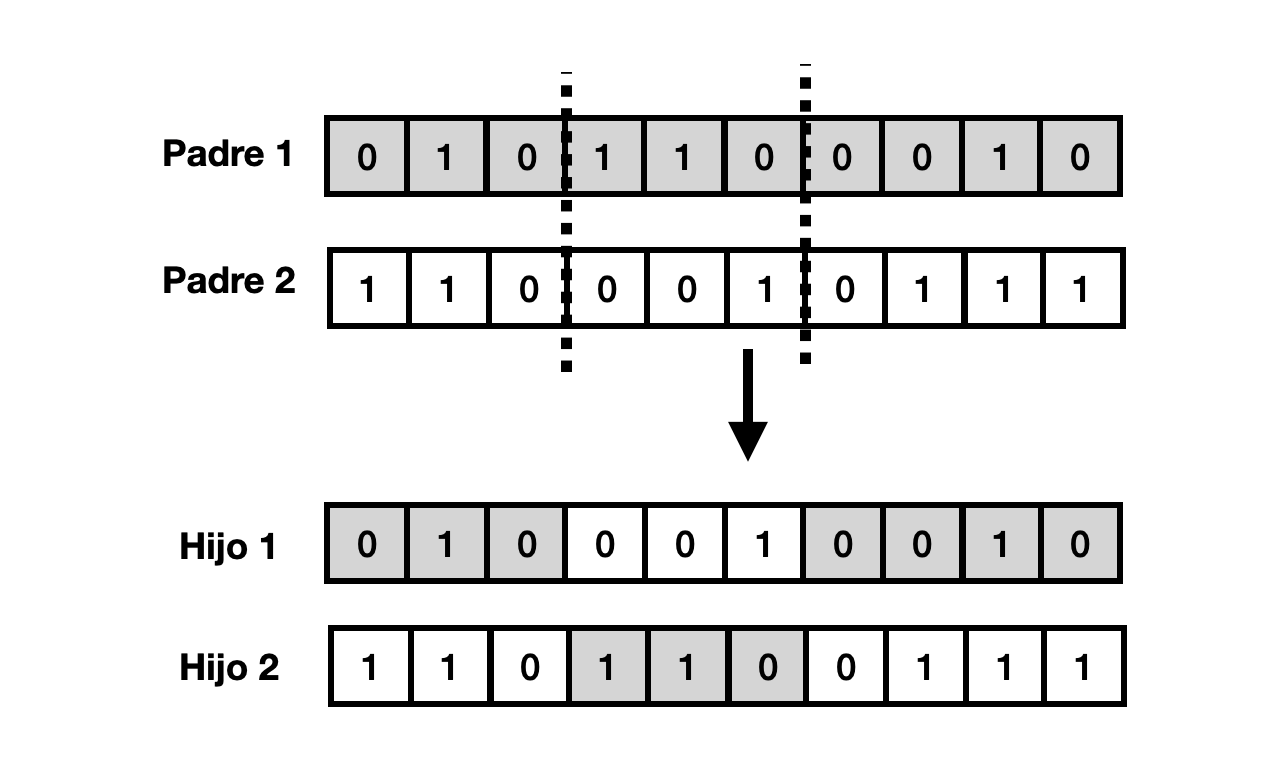
\includegraphics[width=0.9\textwidth]{images/crossOver.png}
  \caption{Ejemplo de crossover de dos puntos con dos cromosomas.}
  \label{fig:crossover}
\end{figure}

\cacho{Ejemplos de secuencias de metodos}

\pp{Qué significa el crossover para builders?}

En nuestro algoritmo, utilizamos una tasa de cruzamiento de 0.30 (\emph{crossover rate}), lo cual significa que en cada generación aproximadamente el 30 por ciento de los individuos serán seleccionados para cruzarse y crear nuevos descendientes. Este valor fue obtenido a partir de evaluaciones experimentales que hemos realizado para nuestros casos de estudio.

El cruzamiento es una operación fundamental en los algoritmos genéticos, ya que permite combinar información genética de diferentes individuos y crear mayor diversidad en la población, y es esencial para la búsqueda de soluciones más aptas y para acelerar la convergencia del algoritmo.

\subsubsection{Operadores Genéticos: Mutación}

La mutación es otro operador importante en los algoritmos genéticos. Consiste en introducir cambios aleatorios en los cromosomas de los individuos de la población para diversificar la búsqueda. En el proceso de mutación, cada posición del cromosoma de un individuo tiene una pequeña probabilidad de ser modificada. Esto significa que un bit en el cromosoma puede cambiar de valor de manera aleatoria. Por ejemplo, si estamos representando los cromosomas como vectores de bits, una mutación puede implicar cambiar un 0 por un 1 o viceversa. Este operador de mutación es llamado "mutación por inversión de bits", y es adecuado para individuos codificados en binario como nuestro caso. Un ejemplo de mutación por inversión de bits se muestra en la Figura \ref{fig:mutation}. En este ejemplo, las posiciones 2, 4, 5 y 7 del cromosoma fueron seleccionadas para ser mutadas. \cacho{Los individuos con mayor valor de fitness tienen mayor probabilidad de ser seleccionados para mutar.  Esta estrategia busca preservar los mejores individuos y mantener su calidad mientras introduce aleatoriedad en la población.}

\begin{figure}[t]
\centering
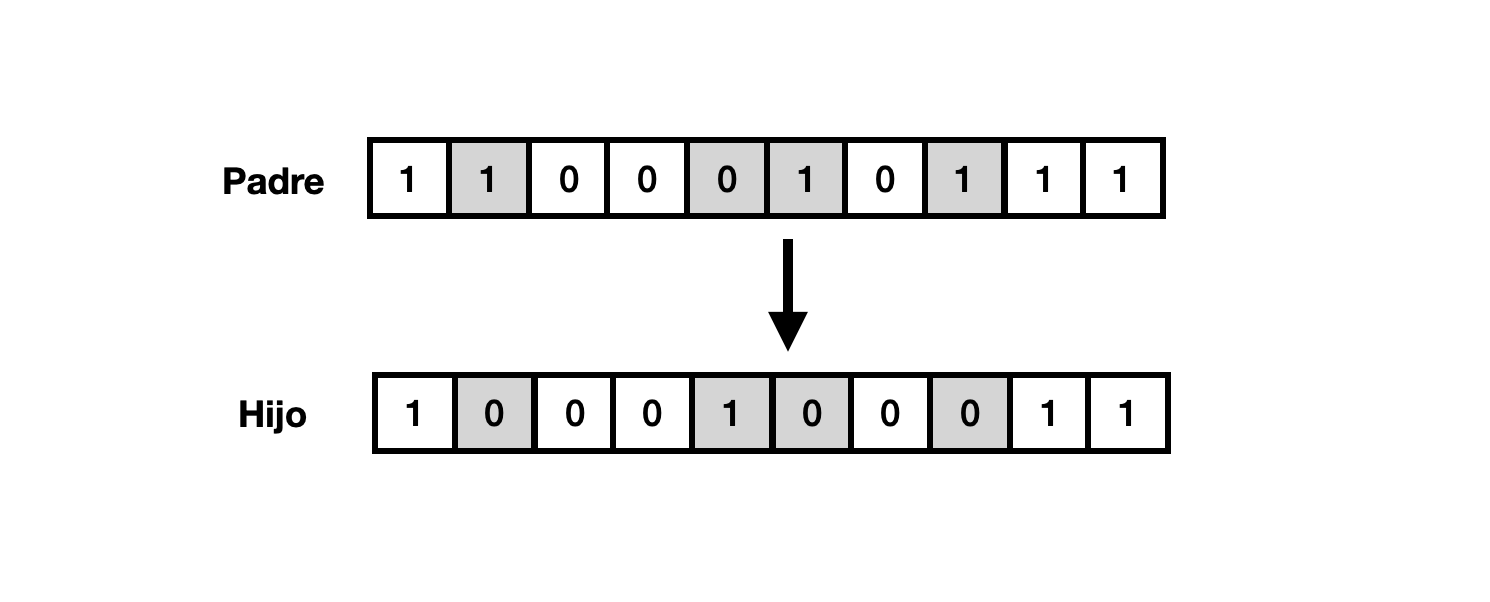
\includegraphics[width=0.9\textwidth]{images/mutation.png}
\caption{Ejemplo de mutación por inversión de bits.}
\label{fig:mutation}
\end{figure}

\pp{Falta describir como se seleccionan los individuos que se van a mutar.}
Aunque la mutación es un proceso aleatorio, la probabilidad de mutar cada bit suele ser pequeña, para evitar que los cambios sean demasiado drásticos y permitir que los individuos más aptos dominen la población. En nuestro algoritmo utilizamos una probabilidad de mutación de 0.05. Esto es, dado un individuo hay un 5\% de probabilidad de mutar el valor de cada bit del cromosoma. Nuevamente, este valor fue obtenido luego de un análisis experimental. Esta alteración aleatoria introduce cambios sutiles en la información del cromosoma, y muchas veces permite crear nuevos descendientes que no estaban presentes en la población original.

El proceso de mutación es crucial para mantener la diversidad genética en la población y permitir que el algoritmo continúe explorando diferentes regiones del espacio de búsqueda. Sin la mutación, el algoritmo genético podría converger rápidamente hacia una solución subóptima y no ser capaz de encontrar soluciones más prometedoras. La combinación de los operadores de selección, cruzamiento y mutación es lo que permite a los algoritmos genéticos encontrar soluciones óptimas o cercanas a las óptimas en problemas complejos de optimización y búsqueda.

\pp{Qué significa la mutación para builders?}

\cacho{La mutación en el contexto de los métodos generadores de objetos es un mecanismo que permite introducir variaciones aleatorias en los estados (conjuntos de métodos). Esto es importante ya que fomenta la exploración de nuevas soluciones y evita que el proceso evolutivo quede atrapado en óptimos locales.}


\subsubsection{Pseudocódigo del algoritmo genético}

La Figura~\ref{lst:genetic_algorithm} muestra un pseudocódigo del algoritmo genético que definimos para la búsqueda de métodos generadores de objetos.

\begin{figure}[H]


\begin{lstlisting}[style=javaStyle, caption={Algoritmo genético en Java}, label={lst:genetic_algorithm}]
public Estado algoritmoGenetico(poblacion, funObjectivo) {
    do {
        Poblacion newPopulation = new Poblacion();
        for (int i = 0; i < poblacion.size(); i++) {
            x = seleccion(poblacion, funObjectivo);
            y = seleccion(poblacion, funObjectivo);
            hijo = cruzamiento(x, y);
            if (mutationProbabilidad) {
                hijo = mutacion(hijo);
            }
            newPopulation.add(hijo);
        }
        poblacion = newPopulation;
    } while (!condicionDeTerminacionCumplida);
    
    return mejorEstadoEnPoblacion(poblacion, funcionValoracion);
}
\end{lstlisting}
\end{figure}

El algoritmo comienza con una población inicial de individuos, que son configuraciones del problema que estamos tratando de resolver. \pp{Antes se menciona que se genera aleatoriamente, no está en el algoritmo esto. Hay que hacer referencia a las secciones en las que se explica cada componente.}.

El algoritmo se ejecuta en ciclos repetitivos llamados generaciones. En cada generación, se crea una nueva población a partir de la población anterior mediante una combinación de selección, cruzamiento y mutación.

En la fase de selección (línea 5 y 6), se eligen los individuos de la población actual que participarán en la reproducción.
Los individuos más aptos, es decir, aquellos con una mayor adaptación o valor de la función objetivo, tienen más probabilidad de ser seleccionados.
En la fase de cruzamiento (línea 7), se seleccionan dos individuos padres de la población y se combinan partes de sus genes para crear nuevos individuos hijos, tal cual lo explicamos en la sección de cruzamiento. \pp{No está en crossover rate.}

Luego, en la fase de mutación (Línea 8 y 9), se introducen cambios aleatorios en los genes de algunos individuos para diversificar la población y evitar que el algoritmo quede atrapado en óptimos locales. La probabilidad de mutación suele ser baja, por ende, depende de esta probabilidad para realizar la mutación.

Una vez que se ha creado la nueva población (Línea 13), reemplaza a la población anterior y se repite el proceso para generar una nueva generación. El algoritmo se repite durante un número determinado de generaciones o hasta que sé durante 7 generaciones se repita siempre el mejor estado \emph{condicionDeTerminacionCumplida} en el algoritmo).
\cacho{Hace falta esto?}\pp{Si, no está en el algoritmo esto}.

Al final del algoritmo, se selecciona el mejor individuo (de acuerdo a la función de valoración) de la última población como la solución encontrada. (Línea 16)

\pp{Acá habría que describir la biblioteca utilizada y meter una referencia}
\cacho{Para implementar el algoritmo genético, utilizamos una biblioteca muy popular en Java llamada \emph{Jenetics}\footnote{https://jenetics.io/}. Esta biblioteca está diseñada específicamente para algoritmos evolutivos y nos proporcionó las herramientas necesarias para desarrollar nuestro enfoque genético.}

\cacho{\emph{Jenetics} es una biblioteca robusta y versátil que ofrece una amplia gama de funcionalidades para la implementación de algoritmos genéticos. Nos permitió definir y manipular genes, cromosomas y poblaciones, así como utilizar operadores genéticos como selección, cruzamiento y mutación. Además, cuenta con un sólido conjunto de herramientas de optimización y técnicas de evolución que nos permitieron adaptar el algoritmo a nuestras necesidades específicas.
Gracias a \emph{Jenetics}, pudimos implementar el algoritmo genético de manera eficiente y efectiva, lo que nos permitió explorar y encontrar subconjuntos óptimos de métodos \emph{builders} para las diferentes estructuras de datos en nuestro estudio. Además, \emph{Jenetics} es muy fácil de usar, con una documentación completa y una comunidad activa de usuarios que proporciona soporte y ayuda. }
\subsection{Algortimo hill climbing}
\label{alg:approachHC}

El algoritmo de escalada (\emph{hill climbing} en inglés) \cite{Russell:2009, Cormen2009, kleinberg2006}, es un algoritmo de búsqueda local que intenta encontrar una solución que maximice (o minimice) el valor de una función objetivo. Su enfoque se basa en realizar siempre movimientos ascendentes, es decir, buscar sucesores del estado actual que mejoren el valor de la función objetivo. La búsqueda de escalada es un algoritmo codicioso (\emph{greedy}), ya que selecciona un estado en base a los sucesores del estado actual (información local) sin tener en cuenta la mejor solución global al problema. A pesar de su simplicidad, los algoritmos codiciosos suelen dar buenas soluciones para algunos problemas. Sin embargo, en algunos casos pueden quedar estancados en un máximo (mínimo) local, y no retornar la solución óptima.

% La búsqueda de escalada a menudo avanza rápidamente hacia una solución porque generalmente es bastante fácil mejorar un estado malo.
% Pero desafortunadamente, la búsqueda de escalada a menudo queda atrapada por las siguientes razones:
% \begin{itemize}
% \item Máximos locales: un máximo local es una cumbre que es más alta que cada uno de sus estados vecinos, pero más baja que el máximo global. Los algoritmos de búsqueda de escalada que llegan a la cercanía de un máximo local serán atraídos hacia la cumbre pero luego se quedarán sin otro lugar adónde ir. 
% \item Crestas: resultan en una secuencia de máximos locales que es muy difícil de navegar para los algoritmos codiciosos.

% \item Mesetas: una meseta es una zona plana del paisaje del espacio de estados. Puede ser un máximo local plano, desde el cual no existe una salida ascendente, desde el cual es posible el progreso. Una búsqueda de escalada puede perderse en la meseta.
% \end{itemize}



\subsubsection{Pseudocódigo}

En esta sección, presentamos un enfoque para la identificación de métodos generadores de objetos basado en un algoritmo de escalada. El pseudocódigo de este enfoque se muestra en la Figura~\ref{alg:hill_climbing}.
La representación que hemos utilizado del problema es la explicada en la sección \ref{sec:estados}. Esto quiere decir que utilizamos vectores de bits para representar los estados. 


\begin{lstlisting}[style=javaStyle, caption={Algoritmo de Hill Climbing}, label={alg:hill_climbing}]
public Estado hillClimbing(problem, funObjectivo) {
    Estado curr = generarEstadoIncial(problem,funObjectivo);
    curr = problem.estadoInicial;
    do {
        List<Estado> sucesores = generarSucesores(curr);
        Estado best = mejorSucesor(sucesores,funObjectivo);
        if (best.value <= curr.value) {
            return curr;
        }
        curr = best;
    }
}
\end{lstlisting}
\pp{Meter una única figura con todas las funciones así se pueden leer más fácil. El <= de la línea 7 está mal, no? mejorSucesor no está definido. generarEstadoInicial no está definido. Qué es problem?}

La idea principal detrás del algoritmo \emph{hill climbing} (ver Algortimo \ref{alg:hill_climbing}) es comenzar con un estado inicial y, en cada iteración, generar los sucesores de un estado y realizar un movimiento hacia el que tenga el mejor valor de la función objetivo. Este proceso se repite hasta que no se pueda encontrar una solución vecina que mejore el valor actual. En ese punto, el algoritmo se detiene y devuelve la mejor solución encontrada hasta el momento. \pp{Habría que poner qué líneas del algoritmo se corresponden con cada cosa. Y mergear con el párrafo de abajo.}


El algoritmo \ref{alg:hill_climbing} representa el esquema básico de \emph{Hill Climbing}, comienza
calculando la función de valoración de todos los \emph{singletons} (Linea 2, \emph{generarEstadoInical}) solo con los métodos constructores activados (osea con el bit prendido en la posición correspondiente al método constructor de la clase). \pp{Habría que hacer un algoritmo con esto.}. El mejor de los \emph{singletons} (mejor valor de la función objetivo) se establece como el candidato actual $curr$, y \emph{Hill Climbing} inicia un proceso de búsqueda típico e iterativo (Línea 4 a 11). \pp{Esto está al revés, hay que explicar esto primero en el algoritmo, y después lo del proceso iterativo que está en el párrafo de arriba.}

\begin{figure}[H]
\begin{lstlisting}[style=javaStyle, caption={Algoritmo de Hill Climbing}, label={alg:sucessores}]
public List<Estados> generarSucesores(Estado s) {
    List<int[]> sucesores = new ArrayList<>();  
    for (int i = 0; i < s.size(); i++) {
        if (s[i] == 0) {
            Estado sucesor = s.clone();
            sucesor[i] = 1;
            sucesores.add(sucesor);
        }
    }
    return sucesores;
}
\end{lstlisting}
\end{figure}
En cada iteración, \emph{Hill Climbing} generar los sucesores del estado corriente (Línea 5). Esto se puede observar en el algoritmo \ref{alg:sucessores}. Esto, simplemente, genera estados sucesores prendiendo únicamente un bit (poniendo 1) por cada bit apagado (bit en 0). Esto significa que crear un sucesor para nuestro problema es agregar un método al estado corriente. El método \emph{generarSucesores} nos devuelve el conjunto de estados del estado \emph{curr}. \pp{Esto también está desordenado. Habría que poner un ejemplo con figuras para que se entienda bien qué hace.}

% El método que genera los sucesores nos devuelve un conjunto de posibles soluciones que se crean a partir de sumarle un método a la solución óptima corriente ($curr$). Es decir, los sucesores  $S$ generados con \emph{GenerarSucesores(curr)} de un candidato $curr$ son los conjuntos {$curr\cup{mi}$}, para cada $mi$ $\in$ API (Línea 3) \pp{Se podría poner el pseudocódigo de generar sucesores, y quizás poner un ejemplo para que se entienda}.
Sea $best$ el sucesor con valor objetivo más alto (línea 6), si este tiene un valor que es menor o igual al corriente, significa que no hay un sucesor mejor y el algoritmo retorna el estado corriente (Línea 7 y 8). Se puede observar que este estado es un máximo local y el algoritmo lo encontró.
En caso de que el valor del estado corriente sea menor al mejor sucesor encontrado en la iteración, se reemplaza el corriente y vuelve a ejecutar una nueva iteración con este estado hasta encontrar un máximo local. \pp{Esto también está explicado arriba, y ahora de nuevo. Hay que ordenarlo.}
% Observe que $best$ tiene exactamente un método más que el mejor candidato de la iteración anterior, $curr$ (Línea 4) \pp{hay que implementar con código el existe un mejor candidato. Mirar el libro de AI.}.

%Se puede observar que este algoritmo puede quedar atrapado en un máximo local y no generar alguna combinación específica que podría ser aún mejor. Aquí se puede ver que es un algoritmo perezoso, ya que obtiene una solución rápida, pero puede no ser eficaz en encontrar la mejor solución global. 

%\subsubsection{Clases de equivalencia}
%\label{alg:approachCE}
 %Las clases de equivalencia son una técnica utilizada para agrupar conjuntos de datos de entrada en categorías o clases que tienen un comportamiento similar o producen resultados equivalentes. Esta técnica es ampliamente utilizada en el diseño y la realización de pruebas de software.
 %En términos generales, una clase de equivalencia representa  un conjunto de que se espera que produzcan resultados idénticos. La idea es que si un conjunto de la clase de equivalencia produce un resultado, entonces todas las demás entradas de esa clase deberían producir el mismo resultado.
 %Al trabajar con clases de equivalencia, se selecciona una entrada representativa, llamada caso de prueba, de cada clase para ser evaluada. En lugar de probar todas las posibles entradas, se eligen casos de prueba que representen cada clase de equivalencia para minimizar la cantidad total de pruebas necesarias.

 %Bajo esta introducción, hemos desarrollado un tercer algoritmo donde agrupamos en clases de equivalencia aquellos subconjuntos de métodos que tengan el mismo valor de la función objetivo con alguna de las funciones explicadas en \ref{sec:fitness}.

%\subsection{Pseudo-Código}

%\begin{figure}[H]
%\begin{lstlisting}[style=javaStyle, caption={Algoritmo basado en Clases de Equivalencia}, label={algo:clases_equivalencia}]
%public Estado clasesDeEquivalencia() {
%    Estado curr = generarEstadoIncial(problem,funObjectivo);
%    Map<Key, Estado> equivalenceClasses = crearClasesDeEquivalencia(curr);

%    boolean newClassCreated;
%    do {
%        newClassCreated = false;
%        Set<Estados> newCandidates = candidatosPorClase(equivalenceClasses);

%        for (Estado candidate : newCandidates) {
%            Queue<Estado> successors = generarSucesores(candidate);
%            for (Estado successor : successors) {
%                Double key = successor.value;
%                equivalenceClasses.get(key).add(successor);
%                newClassCreated = true;
%            }
%        }
%    } while (newClassCreated);

%    Set<Estado> best = obtenerMejor(equivalenceClasses);
%    return best;
%}
%\end{lstlisting}
%\end{figure}


%En este algoritmo, se comienza obteniendo los conjuntos \emph{singletons} (Línea 1), que son los métodos constructores individuales de la misma manera que el algoritmo de \ref{alg:hill_climbing}. Esto es nuestro estado inicial del algoritmo. A partir de estos singletons, se crea una clase de equivalencia con la \emph{key} que es la función de valoración de cada estado inicial y se agrupan los estados que tienen el mismo valor de valoración. Esto servirá como punto de partida de nuestro algoritmo. (Línea 3).  En el algoritmo las clases de equivalencias están guardadas en $equivalenceClasses$.

%Luego comienza la etapa iterativa (Línea 6 a 18) mientras se haya creado una nueva clase de equivalencia. En cada iteración, se generan nuevos candidatos por cada clase de equivalencia. Es decir, se selecciona un candidato de cada clase de equivalencia (el que tenga menor cantidad de métodos y menor cantidad de parámetros) $candidatosPorClase(equivalenceClasses)$ y se lo guarda en una cola ($newCandidates$) (Línea 8). A continuación, se generan los sucesores (línea 10 y 11) para cada candidato elegido, $GenerarSucesores(candidate)$, utilizando el mismo enfoque que en el algoritmo \ref{alg:sucessores}. Estos se guardan en $successors$. Es decir, si tenemos $N$ clases de equivalencias vamos a tener $N$ candidatos a los cuales le vamos a calcular sus sucesores.  Luego, por cada uno de estos sucesores se le calcula su función de valoración y de acuerdo a esta se lo guarda en la clase de equivalencia representada por el valor de valoración (Línea 14).
%El algoritmo itera hasta que no hayamos creado una nueva clase de equivalencia. Si no hemos creado una clase de equivalencia nueva, quiere decir que no hay cambios y hemos explorado todas las alternativas posibles. 

%Luego, para obtener el mejor conjunto de métodos generadores de objetos que estamos buscando, accedemos a la clase de equivalencia que tenga la \emph{key} más grande (mejor función de valoración) y obteniendo el representante de ese conjunto que tenga menor método y parámetros. Esto lo realiza el método $obtenerMejor(equivalenceClasses)$



% En la búsqueda de soluciones óptimas mediante algoritmos genéticos u otros algoritmos de búsqueda, la función de valoración \cite{goldberg1989genetic} desempeña un papel fundamental. Su diseño adecuado es crucial, ya que determina la dirección y el éxito del proceso de búsqueda.
% La función de valoración evalúa la calidad de cada solución candidata y la compara con otras soluciones en la población. Proporciona una medida objetiva de la idoneidad de cada individuo en relación con los objetivos y restricciones del problema. La calidad se expresa generalmente mediante un valor numérico, donde valores más altos indican soluciones más deseables. Por ejemplo, si estamos resolviendo un problema de optimización en el que buscamos maximizar una función objetivo, la función de valoración puede asignar un valor más alto a las soluciones que se acercan más a la solución óptima. Por otro lado, si estamos resolviendo un problema de minimización, la función de valoración puede asignar un valor más alto a las soluciones que se alejan más de la solución óptima.
% Definir una buena función de valoración implica considerar cuidadosamente los requisitos y características del problema en cuestión. Puede implicar ponderar diferentes objetivos, como maximizar o minimizar ciertas variables, satisfacer restricciones específicas o lograr un equilibrio entre múltiples criterios. 

% Una función de valoración efectiva debe ser capaz de discriminar entre soluciones prometedoras y soluciones subóptimas. Debe proporcionar una evaluación objetiva y precisa, permitiendo la selección de soluciones de alta calidad y la eliminación de soluciones menos deseables.
% Además, la función de valoración debe ser adecuada para el dominio y el tipo de problema abordado. Puede requerir conocimiento especializado y experiencia en el campo para definir correctamente las métricas y ponderaciones apropiadas. 

% Es importante tener en cuenta que la función de valoración puede evolucionar y adaptarse a lo largo del proceso de búsqueda. A medida que el algoritmo de busqueda avanza y produce nuevas generaciones de soluciones, la función de valoración puede ser ajustada y refinada para enfocarse en las características más relevantes y deseadas.


% Por lo tanto, en los algoritmos de búsqueda la función de valoración desempeña un papel crucial para evaluar y comparar soluciones candidatas en función de criterios específicos del problema. Proporciona una medida cuantitativa de la calidad de las soluciones y guía el proceso de selección y toma de decisiones en cada etapa del algoritmo. El diseño adecuado de la función de valoración es esencial para obtener resultados óptimos y eficientes en la resolución de problemas.
% A continuación, explicaremos cada función de valoración implementada en nuestros algoritmos.


% En el caso de algoritmos greedy, la función de valoración juega un papel similar pero con un enfoque más local. En lugar de trabajar con una población de soluciones, los algoritmos greedy toman decisiones en cada paso basándose en una evaluación local de las opciones disponibles. La función de valoración en un algoritmo greedy se utiliza para seleccionar la mejor opción en cada iteración o paso del algoritmo, maximizando o minimizando la función de valoración según el objetivo del problema \cite{cormen2009introduction}.



